% Copyright 2004 by Till Tantau <tantau@users.sourceforge.net>.
%
% In principle, this file can be redistributed and/or modified under
% the terms of the GNU Public License, version 2.
%
% However, this file is supposed to be a template to be modified
% for your own needs. For this reason, if you use this file as a
% template and not specifically distribute it as part of a another
% package/program, I grant the extra permission to freely copy and
% modify this file as you see fit and even to delete this copyright
% notice. 

\documentclass{beamer}
% Replace the \documentclass declaration above
% with the following two lines to typeset your 
% lecture notes as a handout:
%\documentclass{article}
%\usepackage{beamerarticle}

\usepackage[utf8x]{inputenc}
\usepackage[spanish]{babel}
\usepackage{fancyvrb}
% \usepackage{verbatim}

% There are many different themes available for Beamer. A comprehensive
% list with examples is given here:
% http://deic.uab.es/~iblanes/beamer_gallery/index_by_theme.html
% You can uncomment the themes below if you would like to use a different
% one:
%\usetheme{AnnArbor}
%\usetheme{Antibes}
%\usetheme{Bergen}
%\usetheme{Berkeley}
%\usetheme{Berlin}
%\usetheme{Boadilla}
%\usetheme{boxes}
%\usetheme{CambridgeUS}
%\usetheme{Copenhagen}
%\usetheme{Darmstadt}
%\usetheme{default}
%\usetheme{Frankfurt}
%  \usetheme{Goettingen}
%\usetheme{Hannover}
%\usetheme{Ilmenau}
%\usetheme{JuanLesPins}
%\usetheme{Luebeck}
%\usetheme{Madrid}
%\usetheme{Malmoe}
%\usetheme{Marburg}
%\usetheme{Montpellier}
%\usetheme{PaloAlto}
%\usetheme{Pittsburgh}
%\usetheme{Rochester}
\usetheme{Singapore}
%\usetheme{Szeged}
%\usetheme{Warsaw}


\title{Automatización y Scripting}


\begin{document}

\begin{frame}
  \titlepage

\end{frame}





\begin{frame}{}
\frametitle{Variables}
\begin{itemize}
\item Una variable es una marca/etiqueta/identificador/o nombre en el programa, y refiere a una ubicacion de memoria.

\item Algunas variables pueden son definidas por el programador, otras son variables especiales (por ejemplo PATH que es una variable de ambiente).
\item Las nombres de las variables diferencian las mayúsculas de las minúsculas.
\item Los nombres deben comenzar con una letra o guíon bajo \_.
\item El shell de UNIX interpreta los comandos del usuario. Los comandos pueden ser :
\end{itemize}

\end{frame}


\begin{frame}{}
\frametitle{Variables - Continuacion}
Los shell UNIX más avanzados soportan cuatro tipos de datos:
\begin{itemize}
\item Cadenas de caracteres (strings), que son secuencias de caracteres alfanuméricos. 
\item Enteros (Integers), los cuales son números enteros.
\item Punto Flotante (Floats), que son números decimales en punto flotante. 
\item Arreglos (Arays), que son secuencias de variables.
\end{itemize}
\textbf{BASH utiliza cadenas de caracteres y enteros}
\end{frame}{}

\begin{frame}{}
\frametitle{Usando Varibables}
\begin{itemize}
\item       A  una  variable se le puede asignar un valor mediante una sentencia de
       la forma :\\ 
             \texttt{        nombre=[valor]}
\item Para hacer referencia al valor de una variable se utiliza el signo pesos "\$". Ej.:\\
             \texttt{        echo \$HOME}
\item Puede utilizar el símbolo \$ para asignar el valor de una variable a otra variable. EJ.:\\
             \texttt{        casa=\$HOME}
\item Para eliminar una variable se utiliza el comando \texttt{unset}. 

\end{itemize}
\end{frame}{}


\begin{frame}{}
\frametitle{Variables locales y su alcance}
\begin{itemize}
\item El alcance de una variable local está destinado al shell en donde se ha creado la variable. Los procesos hijos no pueden acceder a las variables locales del padre.
\item Una variable puede ser agregada al entorno para ser vista por los procesos hijoas mediante la orden \texttt{export}
\end{itemize}
\end{frame}{}

\begin{Verbatim}

# Variables locales y su alcance

$ TIERRA=mundo	# definicion de una variable local
$ echo $TIERRA	# muestra el contenido de TIERRA
mundo
$ bash		# se inicia un nuevo shell hijo
$ echo $TIERRA	# la variable TIERRA está vacía!
$ exit		# se vuelve al shell anterior
$ echo $TIERRA	# la variable TIERRA aún existe acá
mundo
$ export TIERRA
$ bash		# se inicia un nuevo shell hijo
$ echo $TIERRA	# la variable TIERRA es vista!
mundo
$ EARTH=$TIERRA	# definimos una nueva variable
$ echo $EARTH	# muestra el contenido de EARTH
mundo
\end{Verbatim}

\begin{frame}{}
\frametitle{Comillas}
% Las comillas se utilizan para evitar que el shell procese espacios y caracteres especiales.
\begin{itemize}
\item Las comillas simples (') permiten ocultar el significado de todos los caracteres 
		especiales, o metacaracteres. Incluyendo comillas dobles, 
		invertidas, espacios y saltos de linea. Por este motivo evitan 
		la sustitución de variables y comandos.
\item Las comillas dobles (") permiten ocultar el significado de los caracteres especiales, 
 		espacios y saltos de linea con excepción de las comillas 
 		invertidas, y los caracteres \$ y barra invertida. Permiten la expansión de variables y comandos.
\item
Las Comillas invertidas (`) permiten substituir órdenes con su resultado.
		Cuando encerramos un comando entre comillas invertidas, el shell 
ejecuta y 
		sustituye el comando y las comillas invertidas por el resultado del 
		la ejecución.
\end{itemize}
\end{frame}{}


\begin{Verbatim}

# Comillas - Verificar : 

$ echo '* y $HOME'	# comillas simples
$ echo * y $HOME

$ HOGARYRUTA="$HOME y $PATH"	# comillas dobles
$ echo $HOGARYRUTA
$ NUEVOHOGAR=$HOME y $PATH


$ NOMBRE=`hostname`	# comillas invertidas
$ echo $NOMBRE
$ echo Los siguientes usuarios están online: `who` 

# Puede utilizar tambien $(hostame) en lugar de
# las comillas invertidas!


\end{Verbatim}


\begin{frame}{}
\textbf{Ejecutando un script en BASH }
\begin{itemize}
\item El script debe ser copiado dentro de un directorio de PATH; o
\item debe ser ejecutado con la ruta relativa o completa. Ej. : \texttt{./script.sh}
\item Tambien puede ser ejecutado explicitamente por un shell. Ejemplo : \texttt{bash script.sh}
\end{itemize}

\end{frame}

\begin{frame}{}
\textbf{Algunas prácticas al escribir scripts }
\begin{itemize}
\item Se aconseja explicitamente indicar el shell con \#!
\item Deberia contar con al menos dos tipos de comentarios :
\begin{enumerate}
\item Un comentario al principio del programa script explicando a los usuarios que HACE el script.
\item Comentarios en el código, ya que no somos las únicas personas que leeremos el script 
(los administradores suelen ejecutar y modificar scripts escritos por otros administradores)
\end{enumerate}
\end{itemize}

\end{frame}


\begin{frame}{}
\textbf{Ejemplo de un script escrito en BASH }

\begin{center}
 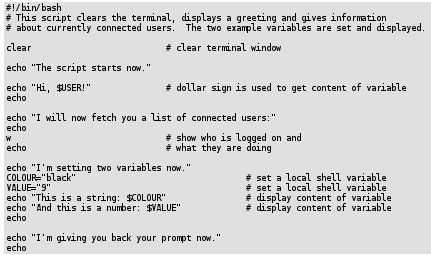
\includegraphics{script2.png}
 % redireccionamiento.gif: 502x248 pixel, 72dpi, 17.71x8.75 cm, bb=0 0 502 248
\end{center}

\end{frame}

\begin{frame}{}
Bibliografía : 
\begin{itemize}
\item man bash
\item Libro Bash Guide for Beginners, de Machtelt Garrels 
\item Libro Advanced Bash-Scripting Guide, de Mendel Cooper
\end{itemize}

Ambos libros están disponibles en varios formatos diferentes en :

Bibliografía suplementaria sugerida : 
\begin{itemize}
\item Libro El Entorno De Programacion Unix, de Kernighan, y Rob Pike
\end{itemize}

\end{frame}



\end{document}


